% Options for packages loaded elsewhere
\PassOptionsToPackage{unicode}{hyperref}
\PassOptionsToPackage{hyphens}{url}
%
\documentclass[
  12pt,
]{book}
\usepackage{amsmath,amssymb}
\usepackage[]{libertinus}
\usepackage{setspace}
\usepackage{iftex}
\ifPDFTeX
  \usepackage[T1]{fontenc}
  \usepackage[utf8]{inputenc}
  \usepackage{textcomp} % provide euro and other symbols
\else % if luatex or xetex
  \usepackage{unicode-math}
  \defaultfontfeatures{Scale=MatchLowercase}
  \defaultfontfeatures[\rmfamily]{Ligatures=TeX,Scale=1}
\fi
% Use upquote if available, for straight quotes in verbatim environments
\IfFileExists{upquote.sty}{\usepackage{upquote}}{}
\IfFileExists{microtype.sty}{% use microtype if available
  \usepackage[]{microtype}
  \UseMicrotypeSet[protrusion]{basicmath} % disable protrusion for tt fonts
}{}
\makeatletter
\@ifundefined{KOMAClassName}{% if non-KOMA class
  \IfFileExists{parskip.sty}{%
    \usepackage{parskip}
  }{% else
    \setlength{\parindent}{0pt}
    \setlength{\parskip}{6pt plus 2pt minus 1pt}}
}{% if KOMA class
  \KOMAoptions{parskip=half}}
\makeatother
\usepackage{xcolor}
\IfFileExists{xurl.sty}{\usepackage{xurl}}{} % add URL line breaks if available
\IfFileExists{bookmark.sty}{\usepackage{bookmark}}{\usepackage{hyperref}}
\hypersetup{
  pdftitle={Marc Nickl},
  hidelinks,
  pdfcreator={LaTeX via pandoc}}
\urlstyle{same} % disable monospaced font for URLs
\usepackage[a4paper,margin=1in]{geometry}
\usepackage{graphicx}
\makeatletter
\def\maxwidth{\ifdim\Gin@nat@width>\linewidth\linewidth\else\Gin@nat@width\fi}
\def\maxheight{\ifdim\Gin@nat@height>\textheight\textheight\else\Gin@nat@height\fi}
\makeatother
% Scale images if necessary, so that they will not overflow the page
% margins by default, and it is still possible to overwrite the defaults
% using explicit options in \includegraphics[width, height, ...]{}
\setkeys{Gin}{width=\maxwidth,height=\maxheight,keepaspectratio}
% Set default figure placement to htbp
\makeatletter
\def\fps@figure{htbp}
\makeatother
\setlength{\emergencystretch}{3em} % prevent overfull lines
\providecommand{\tightlist}{%
  \setlength{\itemsep}{0pt}\setlength{\parskip}{0pt}}
\setcounter{secnumdepth}{-\maxdimen} % remove section numbering
\newlength{\cslhangindent}
\setlength{\cslhangindent}{1.5em}
\newlength{\csllabelwidth}
\setlength{\csllabelwidth}{3em}
\newlength{\cslentryspacingunit} % times entry-spacing
\setlength{\cslentryspacingunit}{\parskip}
\newenvironment{CSLReferences}[2] % #1 hanging-ident, #2 entry spacing
 {% don't indent paragraphs
  \setlength{\parindent}{0pt}
  % turn on hanging indent if param 1 is 1
  \ifodd #1
  \let\oldpar\par
  \def\par{\hangindent=\cslhangindent\oldpar}
  \fi
  % set entry spacing
  \setlength{\parskip}{#2\cslentryspacingunit}
 }%
 {}
\usepackage{calc}
\newcommand{\CSLBlock}[1]{#1\hfill\break}
\newcommand{\CSLLeftMargin}[1]{\parbox[t]{\csllabelwidth}{#1}}
\newcommand{\CSLRightInline}[1]{\parbox[t]{\linewidth - \csllabelwidth}{#1}\break}
\newcommand{\CSLIndent}[1]{\hspace{\cslhangindent}#1}
\usepackage{graphicx}
\usepackage{multibib}
\ifLuaTeX
  \usepackage{selnolig}  % disable illegal ligatures
\fi

\author{}
\date{}

\begin{document}
\frontmatter

\setstretch{1.5}
\mainmatter
\pagenumbering{arabic}

\begin{titlepage}
    \begin{center}
        \vspace*{4cm}
            
  \LARGE
        \textbf{Herzog and Broomfield}
            
 \vspace{0.5cm}
        \Large
        Compare the non-fiction work of any two directors referenced within this unit
            
   \vspace{10cm}
            
\textbf{Marc Nickl}
            
\vfill
            
            
 \vspace{0.8cm}
                        
   \large
        Screen Studies 
        
\today
            
 \end{center}
\end{titlepage}

\setcounter{tocdepth}{3}
\tableofcontents
\pagebreak

\vspace{20pt}

\begin{center}
“An endless struggle with great benefits of satisfaction when you get to the end” (Broomfield, 2017)

\end{center}

\vspace{20pt}

\hypertarget{title}{%
\section{Title}\label{title}}

\hypertarget{subtitle}{%
\subsection{Subtitle}\label{subtitle}}

\hypertarget{one-below-that}{%
\subsubsection{one below that}\label{one-below-that}}

\hypertarget{another-one}{%
\paragraph{another one}\label{another-one}}

\emph{italics} \textbf{bold} 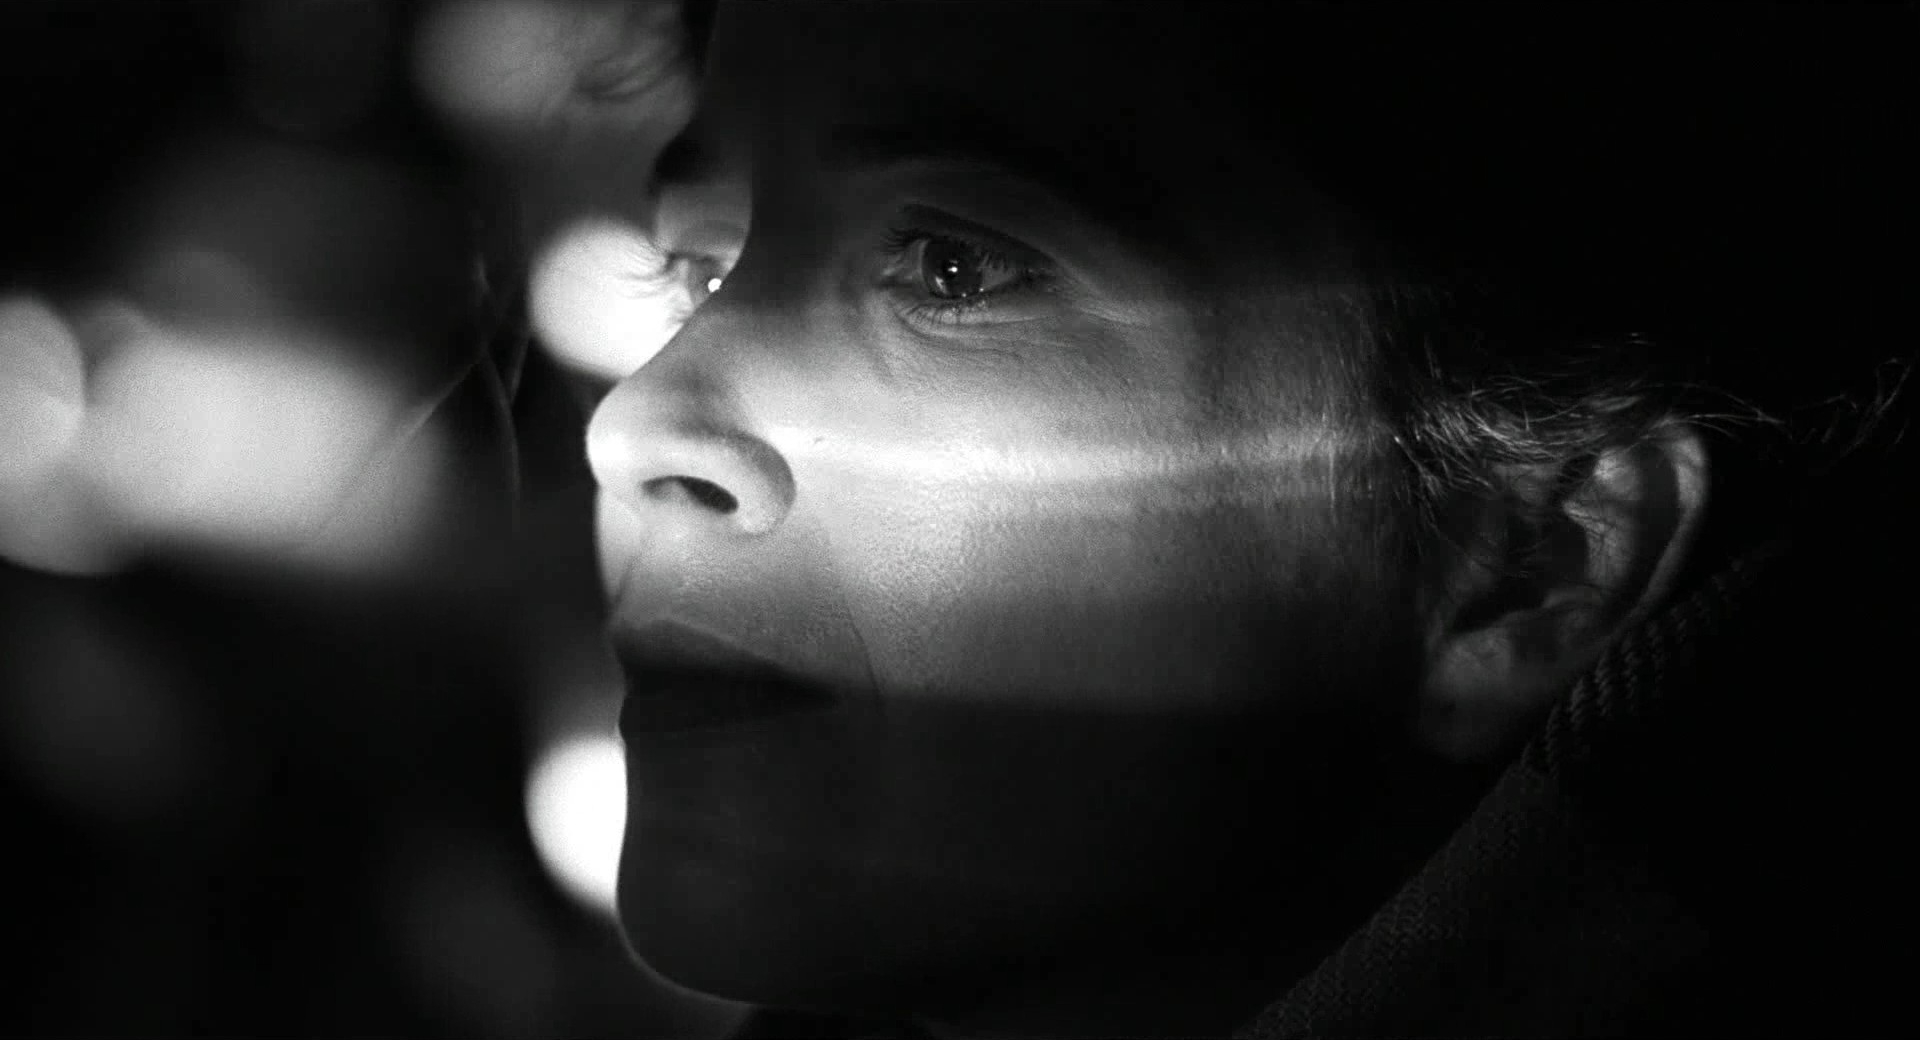
\includegraphics{0314b786c05d34aa190fcc8bf3c6696c.png}

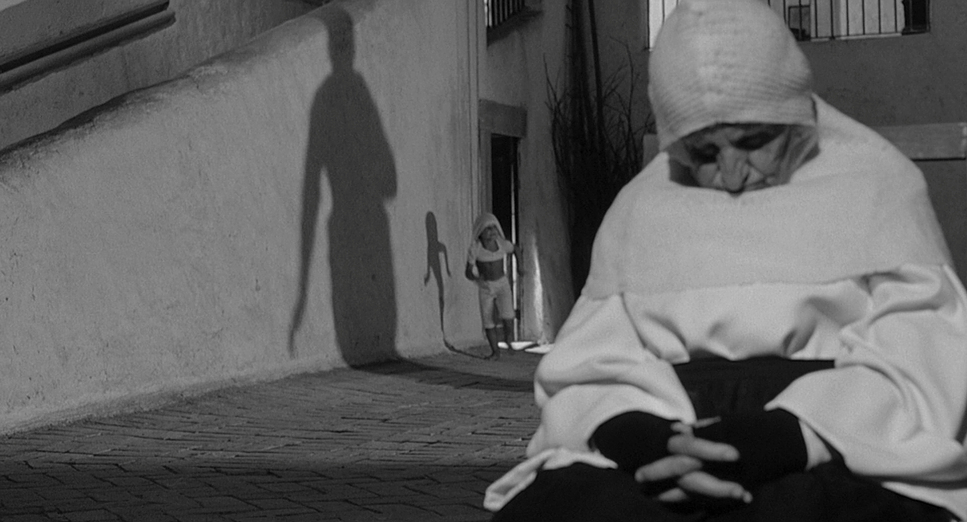
\includegraphics{fd4fef9a20383db8ff25d8806505b409.png} \# This sis for fun

\begin{figure}[ht]

\centering

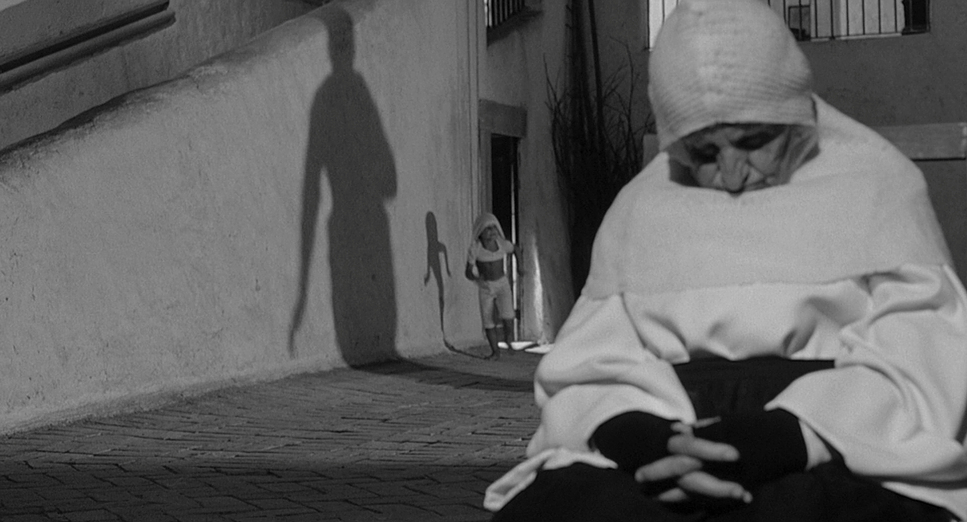
\includegraphics[width=\linewidth]{fd4fef9a20383db8ff25d8806505b409.png}

\caption[Short Title]{\textbf{Short Title:} A long description of the image}

\label{fig:foo}

\end{figure}

This is a sub heading this is the main body of the text

({``Cinematographer Pierre Lhomme on {`Army of Shadows'} - {YouTube}''} 2014) 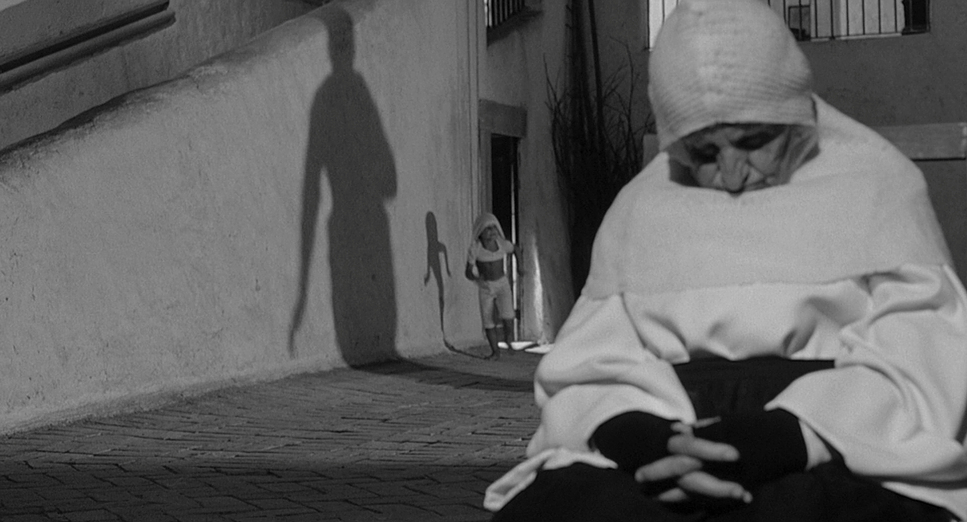
\includegraphics{fd4fef9a20383db8ff25d8806505b409.png}

\textrm{lol }\\
\textsf{ment to be serif }\\
\texttt{text }\\
\textmd{text }\\
\textbf{text }\\
\textup{also not sure }\\
\textit{even less of a clue }\\
\textsl{less clue }\\
\textsc{dont know }\\
\emph{this is an emphasis }\\
\textnormal{text}\{\textbackslash normalfont text\}Document font

\underline{this is underlined }

actors to recreate scenes and Werner Herzog's use of scripting interviews in Lessons in Darkness (2001), where he has ``frontal shots of war victims delivering scripted poetic monologues'' (Peucker 2012, 12)

\hypertarget{List of Illustrations}{%
\chapter{List of Illustrations}\label{List of Illustrations}}

\hypertarget{bibliography}{%
\chapter*{Bibliography}\label{bibliography}}
\addcontentsline{toc}{chapter}{Bibliography}

\hypertarget{refs}{}
\begin{CSLReferences}{1}{0}
\leavevmode\vadjust pre{\hypertarget{ref-noauthor_2014-nk}{}}%
{``Cinematographer Pierre Lhomme on {`Army of Shadows'} - {YouTube}.''} 2014.

\leavevmode\vadjust pre{\hypertarget{ref-Peucker2012-px}{}}%
Peucker, Brigitte. 2012. {``Herzog and Auteurism.''} In \emph{A Companion to Werner Herzog}, 35--57. Oxford, UK: Wiley-Blackwell.

\end{CSLReferences}

\backmatter
\end{document}
